\documentclass{article}

% spelling
\usepackage[english]{babel}

% page layout
\usepackage[letterpaper,top=2cm,bottom=2cm,left=2cm,right=2cm,marginparwidth=1.75cm]{geometry}

% math
\usepackage{amsmath}
\usepackage{amssymb}

% layout
\setlength\parindent{0pt}
\usepackage{setspace}
\usepackage{parskip}
\onehalfspacing
\usepackage{graphicx}

% referencing
\usepackage[colorlinks=true, allcolors=black]{hyperref}
\usepackage[capitalize, nameinlink]{cleveref}
\crefdefaultlabelformat{#2\textbf{#1}#3} % 
\crefname{figure}{\textbf{Figure}}{\textbf{Figures}}
\Crefname{table}{\textbf{Table}}{\textbf{Tables}}

% captions
\usepackage[labelfont=bf]{caption}
\usepackage[table]{xcolor}

% tables
\usepackage{booktabs}
\renewcommand{\arraystretch}{1.25} % vertical spacing


\begin{document}

\begin{titlepage}
        \vspace*{1cm}
            
        \LARGE
        \textbf{Transmission of airborne respiratory infections with and without air cleaners in a school in Switzerland: A modeling study of epidemiological, environmental, and molecular data}
            
        \vspace{0.5cm}
        \Large
        Statistical analysis plan (SAP)
            
        \vspace{1.5cm}
            
        \textbf{SAP authors:} Nicolas Banholzer$^{1*}$, Lukas Fenner$^1$ \\
        \textbf{Study authors:} Nicolas Banholzer$^{1*}$, Philipp Jent$^{2}$, Pascal Bittel$^{2}$, Lavinia Furrer$^{2}$, Tina Hascher$^{3}$, Lukas Fenner$^1$

        \vspace{1cm}

        $^1$ Institute of Social and Preventive Medicine, University of Bern, Switzerland \\
        $^2$ Department of Infectious Diseases, University of Bern, Switzerland \\
        $^3$ Institute of Educational Science, University of Bern, Switzerland \\
        $^*$ Corresponding author: nicolas.banholzer@unibe.ch
            
        \vfill
            
        \Large
        Version number: 0.4 \\
        Version date: \today 

        \vspace*{1cm}
\end{titlepage}

\tableofcontents

\clearpage

\section{Introduction}

This document describes the proposed presentation and analysis for the main paper(s) reporting results from a study estimating and comparing the transmission of airborne respiratory infections with and without air cleaners in schools. To study the effectiveness of air cleaners as an infection control measure, we installed air cleaners in the classrooms of two classes in a secondary school in the Canton of Solothurn, Switzerland (\Cref{fig:study_setting}). Over the study period between January 16 and March 11, 2023, we collected the following data (\Cref{tab:data}):

\begin{enumerate}
    \item \textbf{Molecular data}: Bioaerosol and human saliva samples.
    \item \textbf{Environmental data}: CO$_2$, aerosol and particle concentrations.
    \item \textbf{Epidemiological data}: Daily absences from school.
\end{enumerate}
 
Laboratory and molecular analysis will detect which respiratory infections (e.g. SARS-CoV-2 or Influenza virus) were spreading over the study. Molecular data (positive samples), environmental (particle concentrations), and epidemiological data (absences related to respiratory infections) will then be compared between study conditions with and without air cleaners. The aim of the comparison is to assess whether air cleaners reduced the risk of airborne infection. \smallskip

Any deviations from the statistical analysis plan will be described and justified in the final report. The analysis will be carried out by identified, appropriately qualified, and experienced statisticians, who will ensure the integrity of the data during their processing.

\begin{figure}[!htpb]
    \centering
    \caption{\textbf{Study setting.} Schematic study setup of classrooms where molecular and environmental data were collected. One air cleaner was placed in the front and the other in the back of the classrooms. All devices were placed at the head level of students when they were seated. Both classrooms were not equipped with an active HVAC (Heating, Ventilation, Air conditioning) system, but were ventilated using passive window ventilation.}
    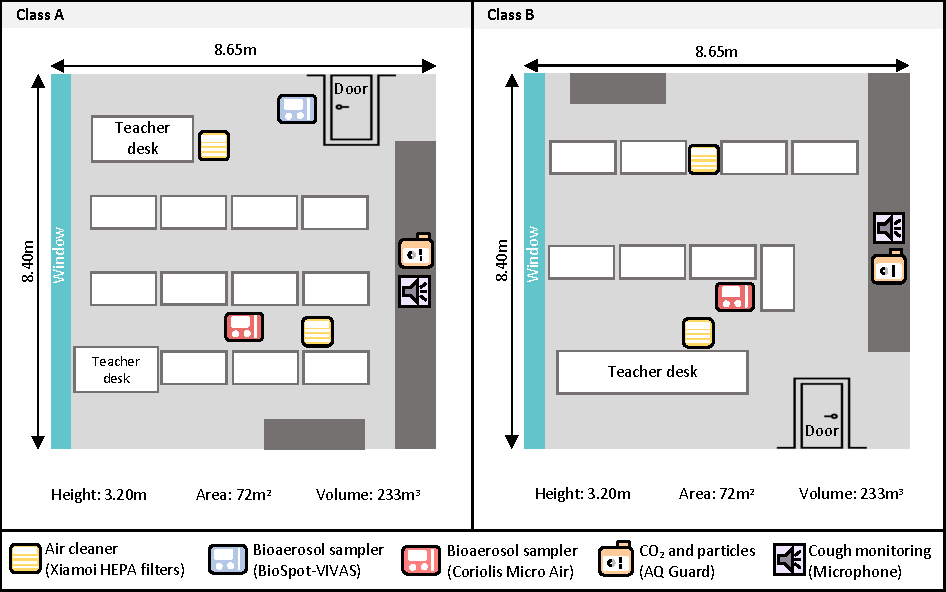
\includegraphics{../study_setting.pdf}
    \label{fig:study_setting}
\end{figure}

\begin{table}[!htpb]
    \footnotesize
    \centering
    \caption{\textbf{Data}. Type of data collected, method/device, and frequency in each class.}
    \begin{tabular}{p{3.5cm}p{6cm} p{1cm} p{1cm} p{3cm}}
    \midrule
    Type of data & Method / device & Class A & Class B & Frequency \\
    \midrule
    \textbf{Molecular data} \\
    \midrule
    Bioaerosol sampling & Bioaerosol sampling devices: BioSpot-VIVAS (Aerosol Devices Inc., Ft. Collins, Colorado, United States) and Coriolis Micro Air (Bertin Instruments Montigny-le/Bretonneux, France) & x & (x) \newline only Coriolis & daily \\
    Saliva samples & Saliva samples & x & x & twice per week \\
    Swabs from air cleaners & Swab samples from Xiaomi HEPA filters (Xiaomi Mi Air Pro 70m2, Shenzhen, China) & x & x & after each intervention phase (both classes) and before the vacation (only class B) \\ 
    \midrule
    \textbf{Environmental data} \\
    \midrule
    CO$_2$, aerosol/particle concentrations, humidity, temperature & Air quality device: AQ Guard (Palas GmbH, Karlsruhe, Germany) & x & x & daily by minute \\
    Coughs & Sounds collected via microphones and coughs detected with a Machine Learning model\cite{Bertschinger2023} & x & x & daily by seconds \\
    \midrule
    \textbf{Epidemiological data} \\
    \midrule
    Absences & Survey & x & x & daily \\
    Student characteristics & Survey & x & x & at study start \\
    \bottomrule
    \end{tabular}
    \label{tab:data}
\end{table}

\section{Background}

In a previous study, we estimated and compared the transmission of airborne infections with and without air cleaners and mask mandates in five classes of two secondary schools in the Canton of Solothurn, Switzerland, between January and March 2022\cite{Banholzer2023}. Air cleaners (commercially available portable HEPA-filtration devices) were found to reduce particle concentrations, but no association was found with transmission. In the previous study, air cleaners were introduced towards the end of the study when most students were already infected with SARS-CoV-2, thus limiting their potential to reduce transmission. By contrast, in this study, we only assess the effectiveness of air cleaners and used a more efficient cross-over design (\cref{tab:study_design}) to assess whether air cleaners are associated with reduced risk of airborne infection in schools.

\begin{table}[!htpb]
    \footnotesize
    \centering
    \caption{\textbf{Study design.} Seven-week study period from January 16 to March 11, 2023, excluding a week of vacation between February 6 and 11. Cross-over design where two portable air cleaners were installed during different time periods in each class (Class A: weeks 1, 2, 6, and 7; Class B: weeks 3, 4, and 5) but not at the same time in both classes.}
    \begin{tabular}{l l l l l l l l l}
    \toprule
      & \textbf{Week 1} & \textbf{Week 2} & \textbf{Week 3} & Vacation & \textbf{Week 4} & \textbf{Week 5} & \textbf{Week 6} & \textbf{Week 7} \\
      & Jan 16-21 & Jan 23-28 & Jan 30-Feb 3 & Feb 6-11 & Feb 13-18 & Feb 20-25 & Feb 27-March 3 & March 6-11 \\
      \midrule
      \textbf{Class A} & \cellcolor{gray!50} Air cleaner & \cellcolor{gray!50} Air cleaner & \cellcolor{gray!10} None & & \cellcolor{gray!10} None & \cellcolor{gray!10} None & \cellcolor{gray!50} Air cleaner & \cellcolor{gray!50} Air cleaner \\
      \textbf{Class B} & \cellcolor{gray!10} None & \cellcolor{gray!10} None & \cellcolor{gray!50} Air cleaner & & \cellcolor{gray!50} Air cleaner & \cellcolor{gray!50} Air cleaner & \cellcolor{gray!10} None & \cellcolor{gray!10} None \\
      \bottomrule
    \end{tabular}
    \label{tab:study_design}
\end{table}

\subsection{Objectives of the study}

The primary objective of the study is to estimate and compare the risk of airborne infection in schools. To this end, the following comparisons between study conditions (with and without air cleaners) are of interest:

\begin{enumerate}
    \item \textbf{Molecular data}: Comparison of positive bioaerosol/saliva samples and viral load concentration.
    \item \textbf{Environmental data}: Comparison of aerosol/particle concentrations.
    \item \textbf{Epidemiological data}: Comparison of the number of infections.  
\end{enumerate}

\subsection{Definitions}

\subsubsection{Case of respiratory infection}

Based on epidemiological data, we will define a case of respiratory infection as an absence where the student reports (a)~a positive lab test result confirming the respiratory infection, or (b)~a sickness with at least one of the following symptoms: fever, coughing, tiredness, loss of test or smell, sore throat, headache, aches and pains, diarrhea, difficulty breathing or shortness of breath, stomach. 

Students were asked to report the first date when they experienced symptoms. For example, a student absent on Monday may report Saturday or Sunday as the symptom onset date. We will denote cases by their symptom onset date. Note that, during the week, the symptom onset date will usually correspond to the absence date, unless the student went to school despite experiencing symptoms.  

\subsection{Primary outcome}

The number of respiratory cases (absences related to respiratory infections by date of symptom onset).  


\subsection{Secondary outcomes}

\begin{enumerate}
    \item The number of positive bioaerosol and saliva samples.
    \item Viral load concentration in positive bioaerosol and saliva samples.
    \item The aerosol/particle number, and matter mass concentrations.
    \item The number of coughs.
\end{enumerate}

\subsection{Variables}

\begin{enumerate}
    \item Molecular data
    \begin{enumerate}
        \item Number and proportion (\%) of positive saliva and bioaerosol samples
        \item Viral load concentration (viral genome load in copies per liter)
        \item Spectrum of viral pathogens detected in bioaerosol and saliva samples, and on the HEPA filters of the air cleaners
    \end{enumerate}
    \item Environmental data 
    \begin{enumerate}
        \item CO$_2$ (parts per million [ppm])
        \item Relative humidity (\%) and temperature (°C)
        \item Particle number (in 1/cm$^3$, particle diameter between 175nm to 20$\mu$m) and matter mass concentrations (PM in $\mu$gm$^{-3}$; PM$_1$, PM$_{2.5}$, PM$_4$, PM$_{10}$, i.e. particles of sizes $<$1 to $<$10$\mu$m)
        \item Number of detected coughs
    \end{enumerate}
    \item Epidemiological data
    \begin{enumerate}
        \item Aggregated (baseline) data per class
        \begin{enumerate}
            \item Number of students per class
            \item Vaccination and recovery status regarding COVID-19 of both students and teachers
            \item Age and gender
        \end{enumerate}
        \item Daily reporting per class
        \begin{enumerate}
            \item Number of absent students and teachers by sex
            \item Reason for absence: sickness, career days, or other
            \item Symptoms: fever, coughing, tiredness, loss of test or smell, sore throat, headache, aches and pains, diarrhea, difficulty breathing or shortness of breath, stomach, or other
            \item Date of symptom onset
            \item Laboratory test performed for respiratory viruses: yes, no, or unknown
            \item Date when the laboratory test was taken
            \item Viruses tested: COVID-19, Influenza A and B, RSV, or other
            \item Laboratory test result: positive or negative
            \item Date when the absent student came back to school
        \end{enumerate}
    \end{enumerate}
    \item Additional data (collected daily at 10min intervals)
    \begin{enumerate}
        \item Working atmosphere: silent working, soft speaking, or loud speaking 
        \item Ventilation: times of window or door opening
        \item Occupancy: breaks, lessons outside the classroom, lessons partly outside the classroom, or school-free hours
    \end{enumerate}
    \item Secondary data
    \begin{enumerate}
        \item Weekly number cases and deaths, laboratory tests and share of positive tests for COVID-19 in the Canton of Solothurn \cite{FOPH2023-cases}
        \item Weekly number of consultations per 100,000 people due to influenza-like illnesses (ILI) \cite{FOPH2023-consultations}
    \end{enumerate}
\end{enumerate}

\subsection{Hypothesis framework}

The null hypothesis will be that there is no true difference in the outcomes between study conditions. We will use a Bayesian framework to assess the null hypothesis and use the posterior distribution of the parameter modeling the difference in the outcome by study condition to assess the direction and magnitude of the effects of air cleaners. 

\section{Study populations}

The target population includes all students from two classes in a secondary school in the Canton of Solothurn, Switzerland. In total, there were 38 students in both classes (Class A: 20, Class B: 18).

\section{Statistical analyses}

\subsection{Comparative analysis}

We will employ descriptive statistics to summarize epidemiological, environmental, and molecular data. Categorical variables will be presented as the number and percentage of students, while continuous variables will be reported with the median and interquartile range (IQR). We will create summary tables to describe student characteristics (age and gender), vaccination status, recovery status, absences, number and share of positive samples, and viral load concentration. We will create figures (box-, bar- and line plots) to compare the share of positive samples, viral load concentration, and particle concentration.

\subsection{Primary analysis}

\subsubsection*{Linking observed cases to unobserved infections}

The number of respiratory cases (absences related to respiratory infections by date of symptom onset) will be modeled with a Bayesian latent hierarchical regression model, which is similar to the model used in our previous study \Cref{Banholzer2023}. The model links the unobserved number of new infections to the observed number of new cases. The number of new cases in class $j$ at time $t$ is modeled with a Negative Binomial distribution   
\begin{align*}
    C_{jt} \sim \text{Negative-Binomial}(\mu_{jt},\phi),
\end{align*}
where $\mu_{jt}$ is the expected number of new cases and $\phi$ is the parameter modeling over-dispersion. The expected number of new cases is the weighted sum of the number of new infections $I_{jt}$ in the  previous days
\begin{align*}
    \mu_{jt} = \sum_{s<t}I_{js} \cdot p_{\text{IN}}(t-s),
\end{align*}
where $p_{\text{IN}}(t-s)$ denotes the probability distribution of the incubation period. The  number of new infections is related to the presence of air cleaners using a log-link
\begin{align*}
    \log I_{jt} &= \log N_{jt} + \beta_0 + \beta_1 \cdot \text{AirCleaner}_{jt} + \beta_2 \cdot \text{Class}_t + \beta_3 \cdot \text{Students}_{jt} + \beta_4 \cdot \text{Ventilation}_{jt} + \beta_5 \cdot \text{CoV}_t + \beta_6 \cdot \text{ILI}_t,
\end{align*}
where $N_{jt} = \sum_{s<t} I_{js}$ is the cumulative number of infections (model offset), $\beta_0$ is the rate of new infections without air cleaners (model intercept), and $\beta_1$ is the effect of air cleaners. The effect of air cleaners will be adjusted for class-specific effects, the number of students in school, the ventilation rate (air changes per hour computed from indoor CO$_2$ levels using the transient mass balance method\cite{Battermann2017}), the proportion of positive tests for SARS-CoV-2 in the community (from secondary data), and the number of consultations for influenza-like illnesses in the community (from secondary data). 

\subsubsection*{Specifying the distribution of the incubation period}

The pathogen of each respiratory infection cannot be identified from the epidemiological data unless students obtained a laboratory test result. As a consequence, different incubation periods will be considered in $p_{\text{IN}}$, reflecting a combination of the pathogen-specific incubation periods. The combination will be determined based on the proportion of positive bioaerosol/saliva samples for each pathogen found in the molecular analysis. The prior distributions for pathogen-specific incubation periods will be based on published estimates. 

\subsubsection*{Adjusting for under-reporting of cases on weekends}

Our previous study recorded a higher proportion of cases on Mondays than on weekends, suggesting recall bias and under-reporting of cases on weekends\cite{Banholzer2023}. To consider weekday effects in the reporting of cases, we will re-weight the expected number of cases each week as follows. Let $k \in $(1: Saturday, 2: Sunday, 3: Monday, $\dots$, 7: Friday) denote the weekday with the week starting on Saturday. The re-weighted expected number of cases $\Tilde{\mu}$ (class and day indexes omitted) are computed as
\begin{align*}
    \Tilde{\mu}_{k} &= \mu_k \cdot \nu_k \cdot \left(\frac{\sum_k \mu_k}{\sum_k \nu_k \cdot \mu_k}\right)\\
    \sum_k \nu_k &= 1,
\end{align*}
where $\nu_k$ is the weight for weekday $k$. These weights will be modeled with a Dirichlet prior
\begin{align*}
    \nu &\sim \text{Dirichlet}(c) \\
    c_k &= \sum_j \sum_t C_{jt} \mathbb{I}_{\text{Weekday}(t)=k}
\end{align*}
where $c_k$ is the total number of cases reported for weekday $k$ and $\mathbb{I}$ is a binary indicator. 

\subsubsection*{Modeling school-free days}

Infections may have occurred during the week of vacation that falls into the study period. The expected number of infections and cases will be computed during vacation, but vacation days are not modeled (i.e. not incorporated into the model likelihood). In addition, we will assume lower transmission of respiratory infections on days without school (weekends and vacations). We incorporate our prior belief into the model intercept $\beta_0$  
\begin{align*}
    \beta_0 &= \alpha + \omega \cdot \text{NoSchool},
\end{align*}
where $\alpha$ is the rate of new infections on school days and $\alpha + \omega$ is the rate on days without school. We will model $\omega$ with an informative prior for a 10\% decrease in new infections on school-free days
\begin{align*}
    \omega &\sim \text{Normal}(\log 1.1, 0.05)~.
\end{align*}

\subsubsection*{Seeding infections before study start}

Cases in the first week of the study could indicate infections before the study commenced. We will therefore seed our model $2 \cdot \text{m}\,$days before the study start, where $\text{m}$ is the average incubation period. The number of infections before the study start will be modeled with an exponential prior
\begin{align*}
    I_{jt} \sim \text{Exponential}(2 \cdot \text{m}) \quad t = -2\cdot\text{m}+1, \dots, 0~. 
\end{align*}

\subsubsection*{Priors for modeling parameters}

Unless stated otherwise, we will use weakly informative priors for all modeling parameters following recommendations on the choice of priors \cite{Gelman2008-Scaling,Gelman2008-Logistic,Gelman2020,Stan2020,Gabry2023}. The continuous adjustment variables will be standardized to have zero mean and a standard deviation of 0.5. 
\begin{align*}
    \alpha &\sim \text{Student-t}_5(0, 10) \\
    \beta_2, \dots, \beta_6 &\sim \text{Student-t}_5(0, 2.5) \\
    \frac{1}{\sqrt{\phi}} &\sim \text{Half-Normal}(0,1),
\end{align*}
All priors represent our default but not definitive choices, and changes in the context of the data will be applied if necessary.


\subsection{Secondary analyses}

\subsubsection{Number of positive bioaerosol and saliva samples}

Molecular analysis will determine whether a bioaerosol or saliva sample is positive for a respiratory pathogen. If a sample is positive for multiple pathogens, we will denote this sample as positive for the pathogen with the highest viral load concentration. Let $p = 0, 1, \dots, P$ denote the pathogen, where $0$ refers to negative samples and $P$ is the number of different pathogens detected over the study. The number of positive bioaerosol and saliva samples $y_p$ in samples of sizes $n$ will be analyzed with a Multinomial logistic regression model
\begin{align*}
    y_0, y_1, \cdots, y_P | n, \beta_0, \beta_1, \beta_2, \beta_3 &\sim \text{Multinomial-Logit}(\theta_0, \theta_1, \dots \theta_P) \\
    \theta &= \text{softmax}(\mu) \\
    \mu &= \begin{cases}
                0, & \text{if } p=0, \\
                \beta_{0[p]} + \beta_{1[p]} \cdot \text{AirCleaner} + \beta_2 \cdot \text{Class} + \beta_3 \cdot \text{Susceptibles}_p, & \text{if } p>0.
            \end{cases} \\
    \beta_0 &\sim \text{Student-t}_5(0, 2.5) \\
    \beta_1 &\sim \text{Normal}(\kappa, \tau) \\
    \kappa, \beta_2, \beta_3 &\sim \text{Student-t}_5\left(0, \frac{2.5}{s_{x}}\right) \\
    \tau &\sim \text{Half-Student-t}_5(0,1),
\end{align*}
where $\text{softmax}(\mu) = \exp(\mu)/\sum\exp(\mu)$, Student-t$_5$ is a Student-t distribution with 5 degrees of freedom, and $s_{x}$ is the empirical standard deviation of each input variable.  Negative tests will be set as the reference category and overall variation in positive samples by pathogen will be modeled with $\beta_0$. The effect of air cleaners will be modeled with a hierarchical prior, where $\kappa$ is the average effect of air cleaners across pathogens and $\tau$ is the variation of the effect between pathogens. The effect of air cleaners will be adjusted for class-specific effects and the decreasing number of susceptibles over time (for each pathogen computed as the number of students minus the total number of positive samples). 

\subsubsection{Viral load concentration in positive samples}\label{subsubsec:viral_load}

Molecular analysis will determine the viral load concentration in positive samples. The viral load concentration in positive samples will be analyzed with a hierarchical linear regression model 
\begin{align*}
    y | \beta_0, \beta_1 &\sim \text{Normal}(\mu,s_{y}) \\
    \mu &= \beta_{0[p]} + \beta_{1[p]} \cdot \text{AirCleaner} \\
    \beta_0 &\sim \text{Normal}(\kappa_0, \tau_0) \\
    \beta_1 &\sim \text{Normal}(\kappa_1, \tau_1) \\
    \kappa_0 &\sim \text{Student-t}_5(\mu_{y}, 2.5s_{y}) \\
    \kappa_1 &\sim \text{Student-t}_5\left(0, 2.5\frac{s_{y}}{s_{x}}\right) \\
    \tau_0, \tau_1 &\sim \text{Half-Student-t}_5(0,1) \\
    \sigma &\sim \text{Exponential}\left(\frac{1}{s_{y}}\right),
\end{align*}
where $\mu_{y}$ and $s_{y}$ are the empirical mean and standard deviation of the outcome. 

\subsubsection{Aerosol/particle concentration}\label{subsubsec:aerosol}

We will only analyze particle concentration data of the time periods during which students were in the classroom. Daily particle concentrations will be summarized with the mean and a log transform will be applied. Each log-transformed particle concentration will be analyzed separately with a linear regression model 
\begin{align*}
    \log y | \beta_0, \beta_1, \dots, \beta_6 &\sim \text{Normal}(\mu,\sigma) \\
    \mu &= \beta_0 + \beta_1 \cdot \text{AirCleaner} + \beta_2 \cdot \text{Class} + \beta_3 \cdot \text{Weekday} + \beta_4 \cdot \text{Students} + \beta_5 \cdot \text{Ventilation} + \beta_6 \cdot \text{Cases}\\
    \beta_0 &\sim \text{Student-t}_5(\mu_y, 2.5s_{y}) \\
    \beta_1, \dots, \beta_6 &\sim \text{Student-t}_5\left(0, 2.5\frac{s_{y}}{s_{x}}\right) \\
    \sigma &\sim \text{Exponential}\left(\frac{1}{s_{y}}\right)~.
\end{align*}
The effect of air cleaners will be adjusted for class- and weekday-specific effects, the number of students in school, the ventilation rate (air changes per hour as computed from indoor CO$_2$ levels), and the cumulative number of cases related to respiratory infections. A log transform will be applied to all continuous input variables. 

\subsubsection{Number of coughs}

The daily number of coughs will be analyzed with a Negative Binomial regression model
\begin{align*}
    y | \beta_0, \beta_1, \dots, \beta_6 &\sim \text{Negative-Binomial}(\mu,\phi) \\
    \log \mu &= \log T + \beta_0 + \beta_1 \cdot \text{AirCleaner} + \beta_2 \cdot \text{Class} + \beta_3 \cdot \text{Weekday} + \beta_4 \cdot \text{Students} + \beta_5 \cdot \text{Ventilation} + \beta_6 \cdot \text{Cases} \\
    \beta_0 &\sim \text{Student-t}_5(0, 2.5) \\
    \beta_1, \dots, \beta_6 &\sim \text{Student-t}_5\left(0, \frac{2.5}{s_{x}}\right) \\
    \frac{1}{\sqrt{\phi}} &\sim \text{Half-Normal}(0,1),
\end{align*}
where $T$ is the daily duration that students were in the classroom and $\phi$ is the parameter modeling over-dispersion in count data. 

\section{Supplementary analyses}

\subsection{Modeling transmission risks}

We will model transmission risks using the Wells-Riley equation\cite{Wells1963} as modified by Rudnick and Milton\cite{Rudnick2003} 
\begin{align*}
    P = \frac{D}{S} = 1 - \exp\left(-\frac{fIqt}{n}\right),
\end{align*}
where $P$ is the risk of infection, $D$ is the number of disease cases, $S$ is the number of susceptibles, $f$ is the fraction of rebreathed air, $I$, is the number of infectious individuals in space, $n$ is the total number of individuals in space, $q$ is the generation rate of infectious quanta (doses of infectious particles), and $t$ is the duration of exposure. Parameters $D$, $S$, and $I$ can be computed based on epidemiological (or molecular) data. The fraction of rebreathed air can be computed from CO$_2$ levels. The number of individuals in space can be determined based on the number of absences. Exposure times can be determined based on the timetable. Thus, we will first use the Wells-Riley equation to estimate the unknown parameter $q$. The risk of infection will then be modeled using the estimated $q$ for exposure times representing a typical school day or week. These risks will be estimated separately for different pathogens detected over the study.  

\subsection{Targeted and deep sequencing}

For positive samples (bioaerosol and saliva samples, swabs from HEPA filters), we will perform targeted sequencing and deep sequencing of viral RNA to compare genetic relatedness between viral strains detected in the air and human samples\cite{Goncalves2021}.

\section{Missing data}

We obtained informed consent from all but one student. As the reason for any absence(s) from this student and the symptoms are unclear, we will consider any absence(s) from this student as unrelated to a respiratory infection. Particle concentrations will be summarized with the daily mean of the minutely values in the time periods when students were in the classroom. Missing values during these time periods will be linearly imputed. Missing values in adjustment variables will be imputed with a fully Bayesian approach where missing values are treated as parameters and a prior is assigned. 

\section{Statistical software employed}

The statistical software R (version 4.2.1 or later) with RStudio will be used for all statistical analyses. Data preprocessing and comparative analyses will be performed in the \texttt{tidyverse} package (version 1.3.2). Bayesian analyses will be performed with the probabilistic programming language Stan (version 2.21.0), using the R interface provided by the \texttt{rstan} package (version 2.21.7), the \texttt{rstanarm} package (version 2.21.3), or the \texttt{brms} package (version 2.18.0).

\end{document}